% =============================================================
%  Supporting validation for the measurement instrument used by
%  every research question in Chapter 6.
% =============================================================

\section{Load-Profile Validation}
\label{sec:results-load-profile-validation}
% Legacy label retained so older cross-references continue to resolve.
\label{sec:results-rq2}

Every goodput number in this chapter comes from the same measurement
instrument: the Explore-and-Refine load profile
(Section~\ref{sec:methods-load-profile}). Before turning to the research
questions, this section checks the properties on which their findings depend.
The profile should return a similar estimate when it measures the same fixed
candidate again, distinguish a transient explore peak from a level the
deployment can sustain, recover from the overload it deliberately induces,
and terminate at a bounded wall-clock cost. These checks validate the
measurement instrument; they are supporting evidence for the research
questions rather than a separate research question about the systems being
optimised.

The phase-level checks use all 632 evaluation runs that reached the bench
stage. The repeatability check uses a separate re-benchmarking campaign in
which every fixed candidate produced by the experiments was measured again,
without changing the candidate between measurements, so that any difference
between the two runs is attributable to the instrument rather than to the
deployment under test.

\begin{table}[H]
  \centering
  \caption{Outcome agreement across the two measurements of each matched
    fixed candidate. A candidate counts as \emph{serving} when the profile
    returns a positive sustained-goodput estimate and as \emph{zero}
    otherwise (Section~\ref{sec:methods-load-profile}). Arrows run from the
    original measurement to the repeat.}
  \label{tab:results-load-profile-concordance}
  \footnotesize
  \begin{tabular}{@{}lrrrrr@{}}
    \toprule
    & & \multicolumn{2}{c}{\textbf{Agree}} & \multicolumn{2}{c}{\textbf{Disagree}} \\
    \cmidrule(lr){3-4}\cmidrule(lr){5-6}
    \textbf{Model} & \textbf{Candidates} & \textbf{Serving} & \textbf{Zero} &
    \textbf{$\to$ zero} & \textbf{$\to$ serving} \\
    \midrule
    \texttt{claude-opus-4-8} & 218 & 146 & 50 & 14 & 8 \\
    \texttt{gpt-5.5}         & 216 & 182 & 23 & 2  & 9 \\
    \texttt{glm-5.2}         & 191 & 109 & 55 & 15 & 12 \\
    \midrule
    \textbf{All}             & 625 & 437 & 128 & 31 & 29 \\
    \bottomrule
  \end{tabular}
\end{table}

\paragraph{Outcome agreement.}
Before comparing magnitudes, the coarser question is whether the two
measurements agree on whether a candidate sustains load at all.
Table~\ref{tab:results-load-profile-concordance} decomposes all 625 matched
candidates on that binary outcome: the two runs agree on $90.4\%$ of them
(Cohen's $\kappa=0.75$). The candidates that report zero twice are
agreement rather than missing data, excluded from the magnitude statistics
below only because a percentage difference between two zeros is undefined.
The 60 disagreements split almost evenly in both directions, which points
to measurement noise near a threshold rather than to drift between the two
campaigns, and they sit low in the goodput range: their positive-side
median is $8{,}056$\,req/s against $18{,}639$\,req/s for candidates
serving in both runs. Agreement is therefore weakest among deployments
already close to failing under load.

\begin{table}[H]
  \centering
  \caption{Repeatability of the sustained-goodput estimate by model, over the
    $n$ candidates that serve in both measurements (the \emph{agree/serving}
    column of Table~\ref{tab:results-load-profile-concordance}). The reported
    statistic is the symmetric percentage difference between the original and
    repeated measurements.}
  \label{tab:results-load-profile-repeatability}
  \footnotesize
  \begin{tabular}{@{}lrrrrr@{}}
    \toprule
    \textbf{Model} & \textbf{$n$} & \textbf{Median} & \textbf{Mean} & \textbf{IQR} & \textbf{P90} \\
    \midrule
    \texttt{claude-opus-4-8} & 146 & $2.6\%$ & $6.9\%$ & $1.1$--$7.3\%$ & $15.8\%$ \\
    \texttt{gpt-5.5}         & 182 & $2.7\%$ & $6.2\%$ & $0.7$--$7.2\%$ & $13.6\%$ \\
    \texttt{glm-5.2}         & 109 & $3.7\%$ & $6.6\%$ & $1.2$--$7.6\%$ & $19.1\%$ \\
    \midrule
    \textbf{All}             & 437 & $2.9\%$ & $6.5\%$ & $1.1$--$7.4\%$ & $15.7\%$ \\
    \bottomrule
  \end{tabular}
\end{table}

\paragraph{Repeatability.}
Restricted to the 437 candidates that return an estimate in both runs,
Table~\ref{tab:results-load-profile-repeatability} shows a typical
difference that is small and consistent across models: the overall median
symmetric difference is $2.9\%$, with a minority of candidates forming a
longer tail that pulls the mean above it, and $90\%$ of the positive pairs
still within $15.7\%$. This is the one place in the chapter that reports an arithmetic
rather than a geometric mean, because the quantity is a measurement error
rather than a goodput level: the geometric mean of these differences is
$2.5\%$, below the median, and would suppress exactly the tail the column is
included to expose. The repeated measurements therefore provide a direct
estimate of the variance attached to the goodput values used in the remaining
sections.

\begin{figure}[H]
  \centering
  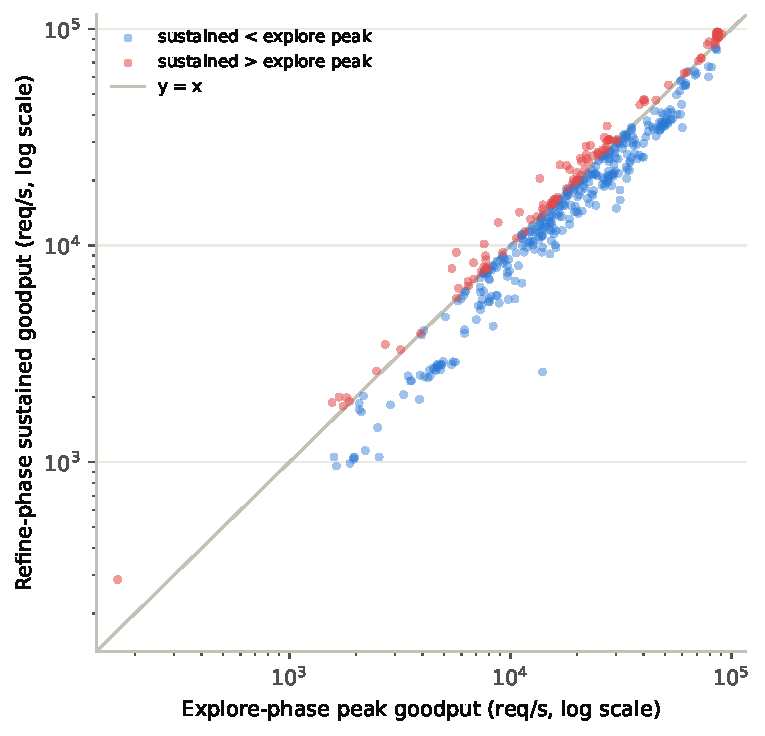
\includegraphics[width=0.62\linewidth]{figures/eval/load_profile_peak_vs_sustained.pdf}
  \caption{Explore-phase peak goodput vs.\ the refine-phase sustained
    estimate, one point per bench run with both quantities defined
    ($n=475$). Points above the $y=x$ line settle higher than their own
    recorded explore peak.}
  \label{fig:results-rq2-peak-vs-sustained}
\end{figure}

\paragraph{Internal consistency.}
Each run yields two goodput figures, explore's transient peak and refine's
sustained estimate, and how they relate shows what refine contributes.
Figure~\ref{fig:results-rq2-peak-vs-sustained} compares them across the 475
runs where both are defined, whose sustained estimates span 287\,req/s to
97{,}138\,req/s, more than two orders of magnitude and the reason explore ramps
exponentially (Section~\ref{sec:methods-load-profile}). Usually refine settles
below the peak (median gap $+10.6\%$, IQR $0.1$--$34.9\%$), since a level
reached while still ramping upward is not one the deployment can hold. In
$24.2\%$ of runs, though, it settles \emph{higher}. In
\texttt{claude-opus-4-8}'s \textsc{Petstore}$\times$\textsc{Go-net-http},
iteration~5, explore stops at 9{,}843 users on a transient p95 spike to
1{,}100\,ms (peak 8{,}801.9\,req/s) while refine settles at
12{,}796.6\,req/s, $1.45\times$ higher. Refine therefore corrects a coarse ramp
that stopped early, rather than only trimming a safety margin off a peak the
profile already trusted.

\begin{table}[H]
  \centering
  \caption{Phase-outcome funnel across all 632 bench runs.}
  \label{tab:results-rq2-funnel}
  \small
  \begin{tabular}{@{}lrr@{}}
    \toprule
    \textbf{Gate} & \textbf{Count} & \textbf{\% of previous stage} \\
    \midrule
    Total bench runs                   & 632 & --- \\
    Survives warm-up                   & 588 & $93.0\%$ \\
    Recovery succeeds                  & 505 & $85.9\%$ \\
    Refine produces an estimate        & 475 & $94.1\%$ \\
    \bottomrule
  \end{tabular}
\end{table}

\paragraph{Reliability and robustness.}
Table~\ref{tab:results-rq2-funnel} follows all 632 runs through the four gates
the profile must clear to report an estimate. Every run that survives the
30-second warm-up health check goes on to trigger one of explore's stop
conditions: $45.6\%$ on a latency breach, $40.0\%$ on a goodput collapse,
and the rest split between a failure-rate breach ($7.0\%$) and the
100{,}000-user ceiling ($7.5\%$). Recovery then hands off to refine in most
of the runs reaching it, and refine produces a usable estimate in all but
30 of those; the 30 enter refine only to hit immediate overload before
completing a single stable settle window, so a successful recovery is not itself
a guarantee that refine will report a nonzero number. Chaining the four gates,
$75.2\%$ of all 632 runs produce a positive sustained-goodput estimate, counted
per bench run rather than per baseline iteration; the rest report exactly $0$
through the failure mechanisms RQ1 describes qualitatively
(Section~\ref{sec:results-rq1}). Where those losses fall argues against the
profile being miscalibrated toward excessive aggression: few runs fail before it
has done anything beyond holding a fixed, modest initial load, and most of the
remaining loss falls at recovery and refine, where a genuinely unhealthy or
regressed deployment would show up regardless of which profile measured it.

\begin{figure}[H]
  \centering
  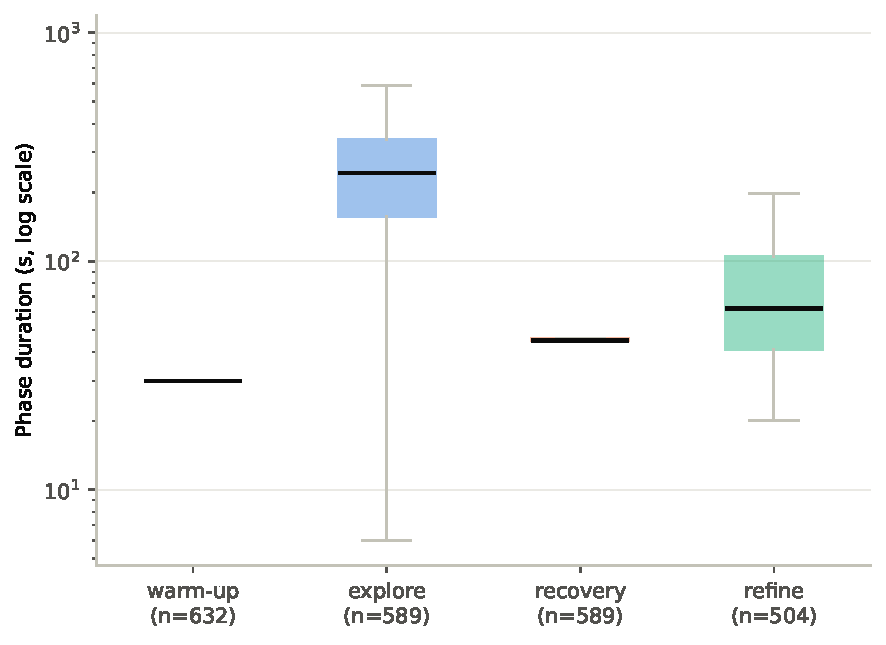
\includegraphics[width=0.72\linewidth]{figures/eval/load_profile_phase_durations.pdf}
  \caption{Wall-clock duration by load-profile phase, across all 632
    individual bench runs in this dataset (log scale; warm-up is
    effectively fixed at 30\,s by construction).}
  \label{fig:results-rq2-phase-durations}
\end{figure}

\paragraph{Bounded wall-clock time.}
A load profile is only usable inside an iterative loop if it locates the
goodput ceiling quickly and within a predictable bound.
Figure~\ref{fig:results-rq2-phase-durations} shows each phase's wall-clock
duration. Warm-up is fixed at 30\,s by construction, and recovery almost always
settles on its first attempt (median 45\,s, matching the profile's settle
window). Explore dominates at a median 242\,s (IQR 157--334\,s), sweeping the
widest range of load levels, while refine takes a median 62\,s (IQR
41--110\,s) despite being the more careful search, because its
efficiency-scaled step size shrinks as the deployment nears its ceiling. A
complete run takes a median of 404\,s (IQR 303--510\,s, maximum 1{,}154\,s):
every one of the 632 runs finished well inside the profile's 30-minute
(1{,}800\,s) budget and stopped on its own phase-completion criteria rather
than on the timeout.

\paragraph{Interpretation.}
Taken together, these checks describe a usable measurement instrument: repeated
measurements agree to within a few percent, the search corrects both optimistic
and prematurely low explore peaks, three in four runs survive the induced
overload to reach an estimate, and every run terminates on its own criteria
inside a fixed budget. These durations measure the instrument's own overhead;
how its search compares against established load-testing profiles remains open.
The sustained-goodput estimate is therefore sound enough to carry the research
questions that follow.
